
This chapter provides detailed specifications of the system under development.

\section{Functional Requirements}

This section describes each function/feature provided by our system. These functions are logically grouped into modules based on their purpose/users/mode of operations etc (as per our system). A functional hierarchy may look like:
\begin{outline}


\1 The system can collect and store data from the black box unit
\1 The system can process and fuse raw data to detect and store driving events
\1 The system should start the ride with the press of a button
\1 The system should end the ride with the press of a button
\1 The system should notify when the ride has started
\1 The system should keep track of the location of the vehicle
\1 The system should present the maneuvers performed by the vehicle at the end of the trip
\1 The system should give the driver their firsts score after completing 40 km of travelling

  
\end{outline}

% --- The above is to be modified as per your project, e.g. a flat list if your system has limited functional requirements.

\section{Non-functional Requirements}

This sections mentions the specific non-functional requirements of our system. These generally address performance, scalability, safety, availability, deployment etc.

\begin{outline}
\1 The system can be operated easily by people without the knowledge about the technology behind it
\1 The system should allow for an easy addition of new components or exchange of existing algorithms
\1 The system should work on its own once the driver presses the start button
\end{outline}

\section{External Interfaces}

\subsection{User Interfaces}

This section includes our mockup screens and briefly explains them.
\\

\begin{center}
    
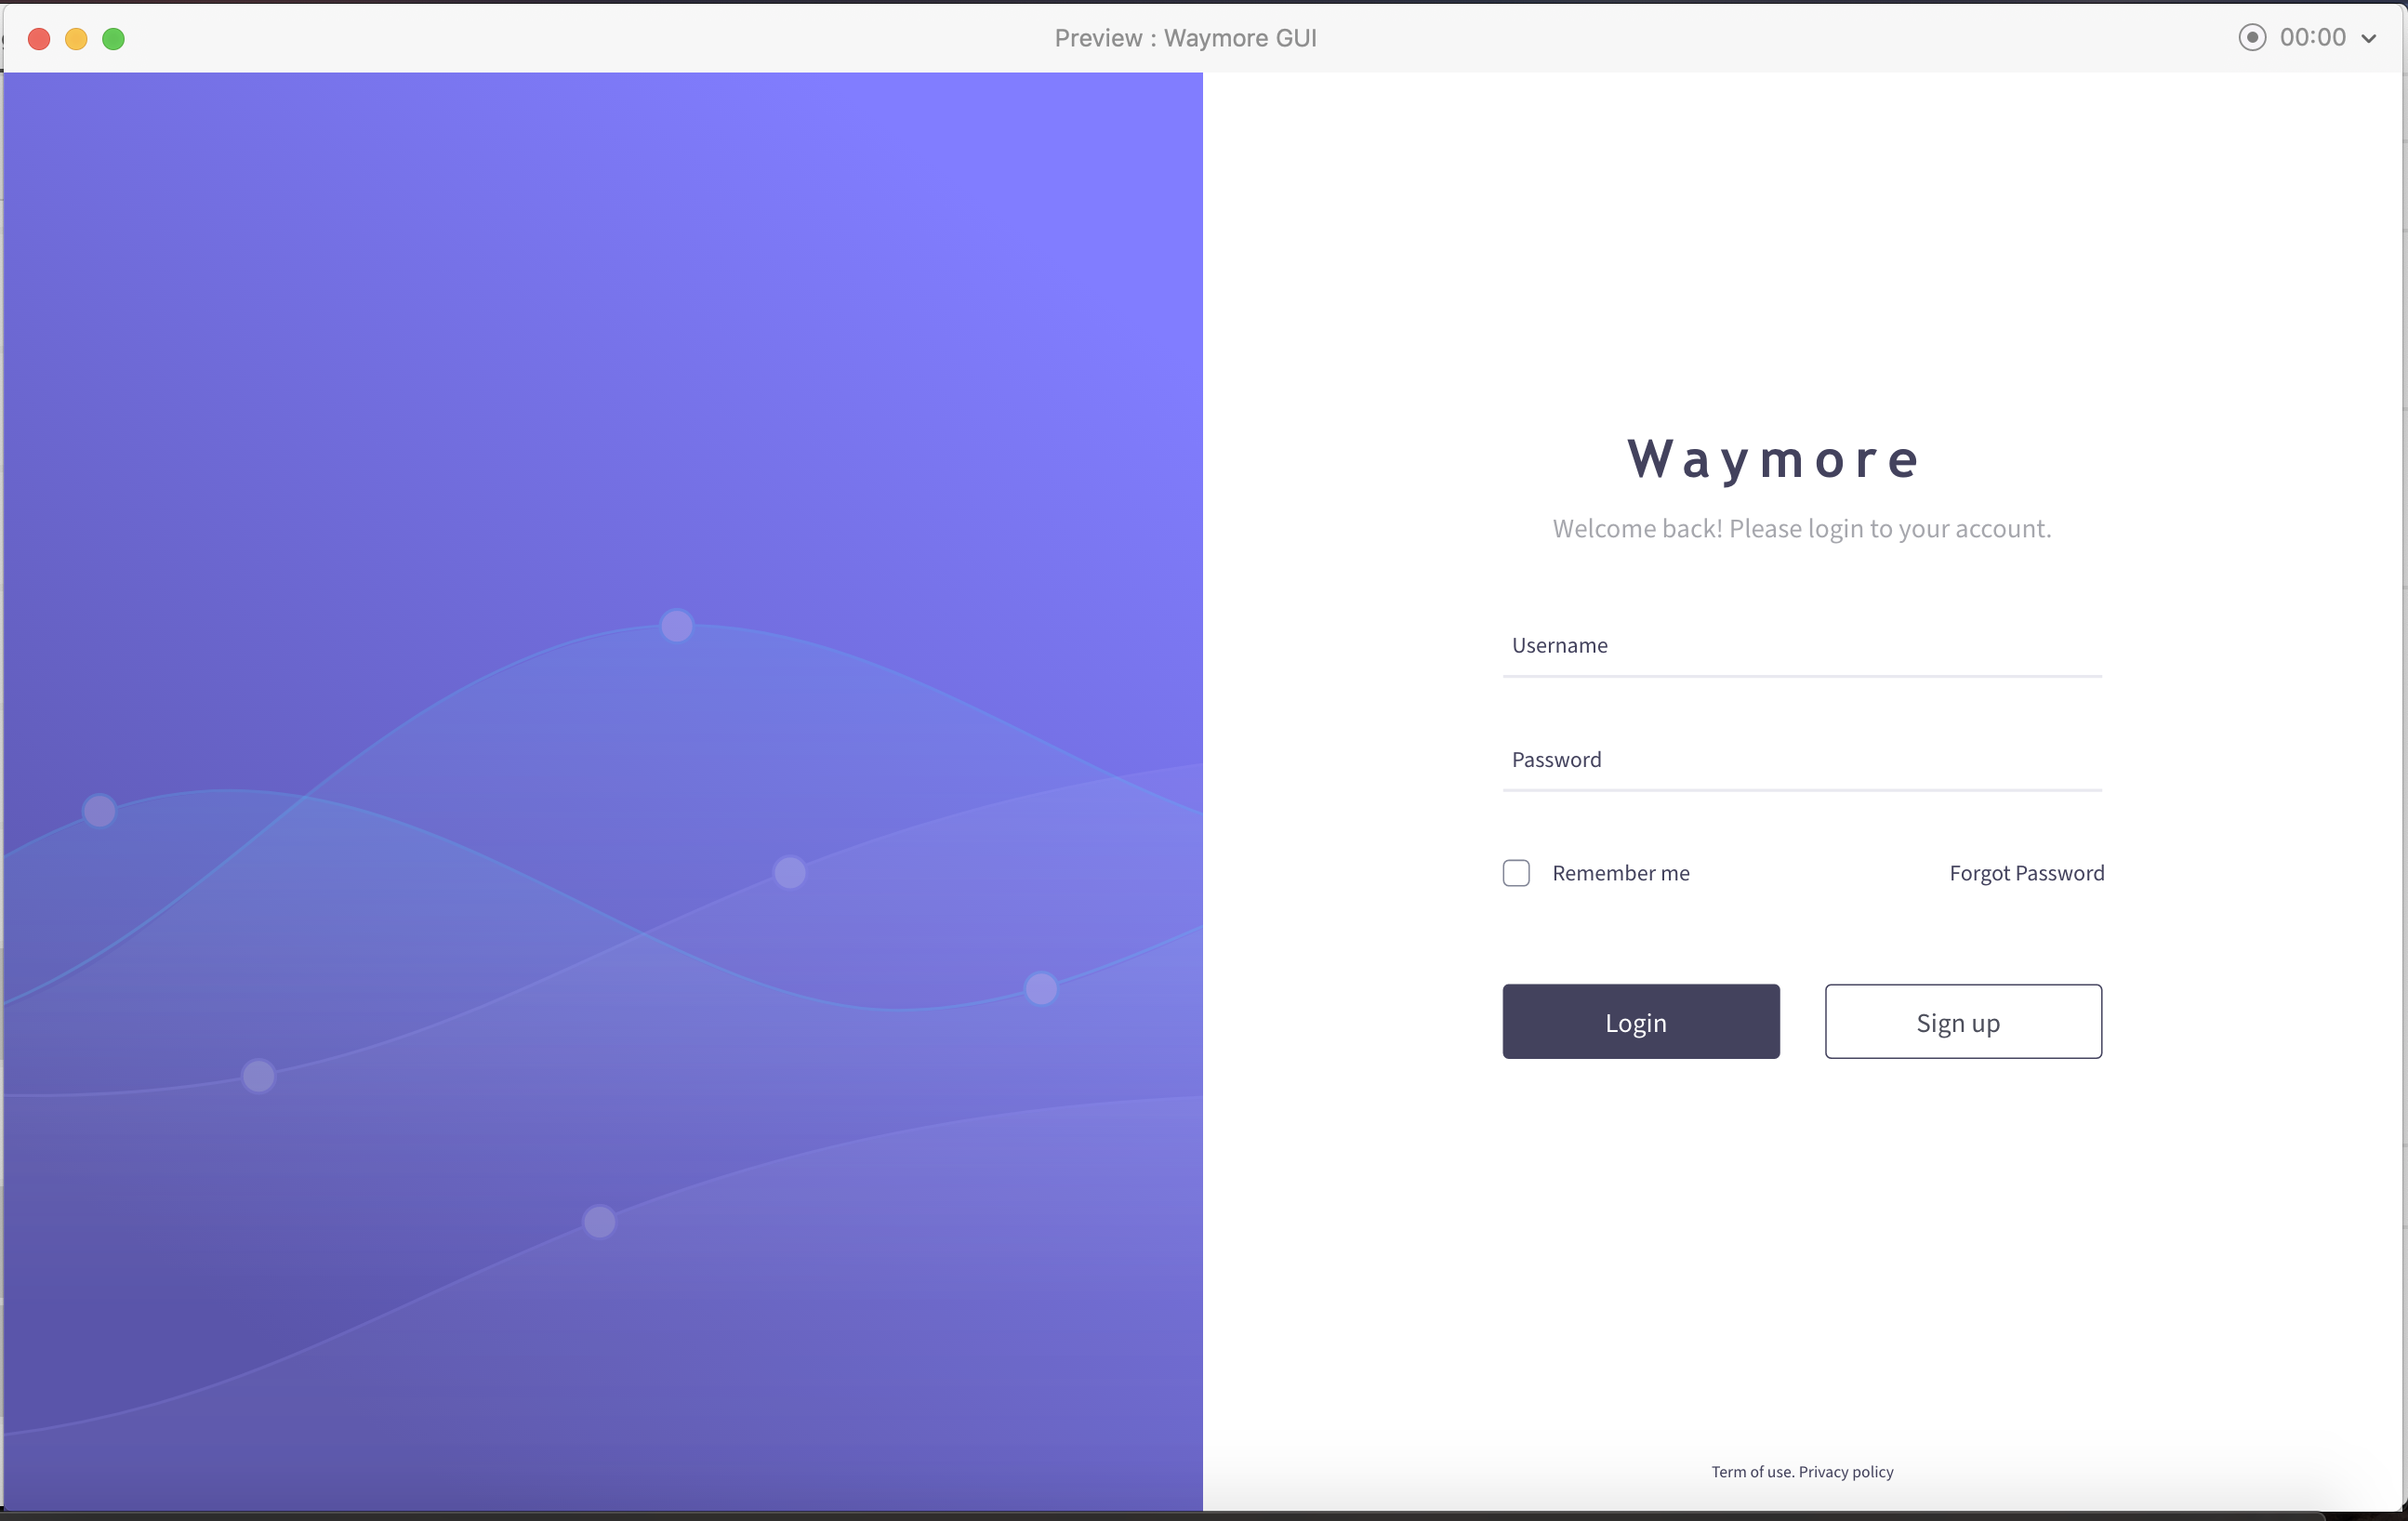
\includegraphics[width = 125mm, scale = 1]{images/1.png}

This screen is the login screen for the user/ stakeholder

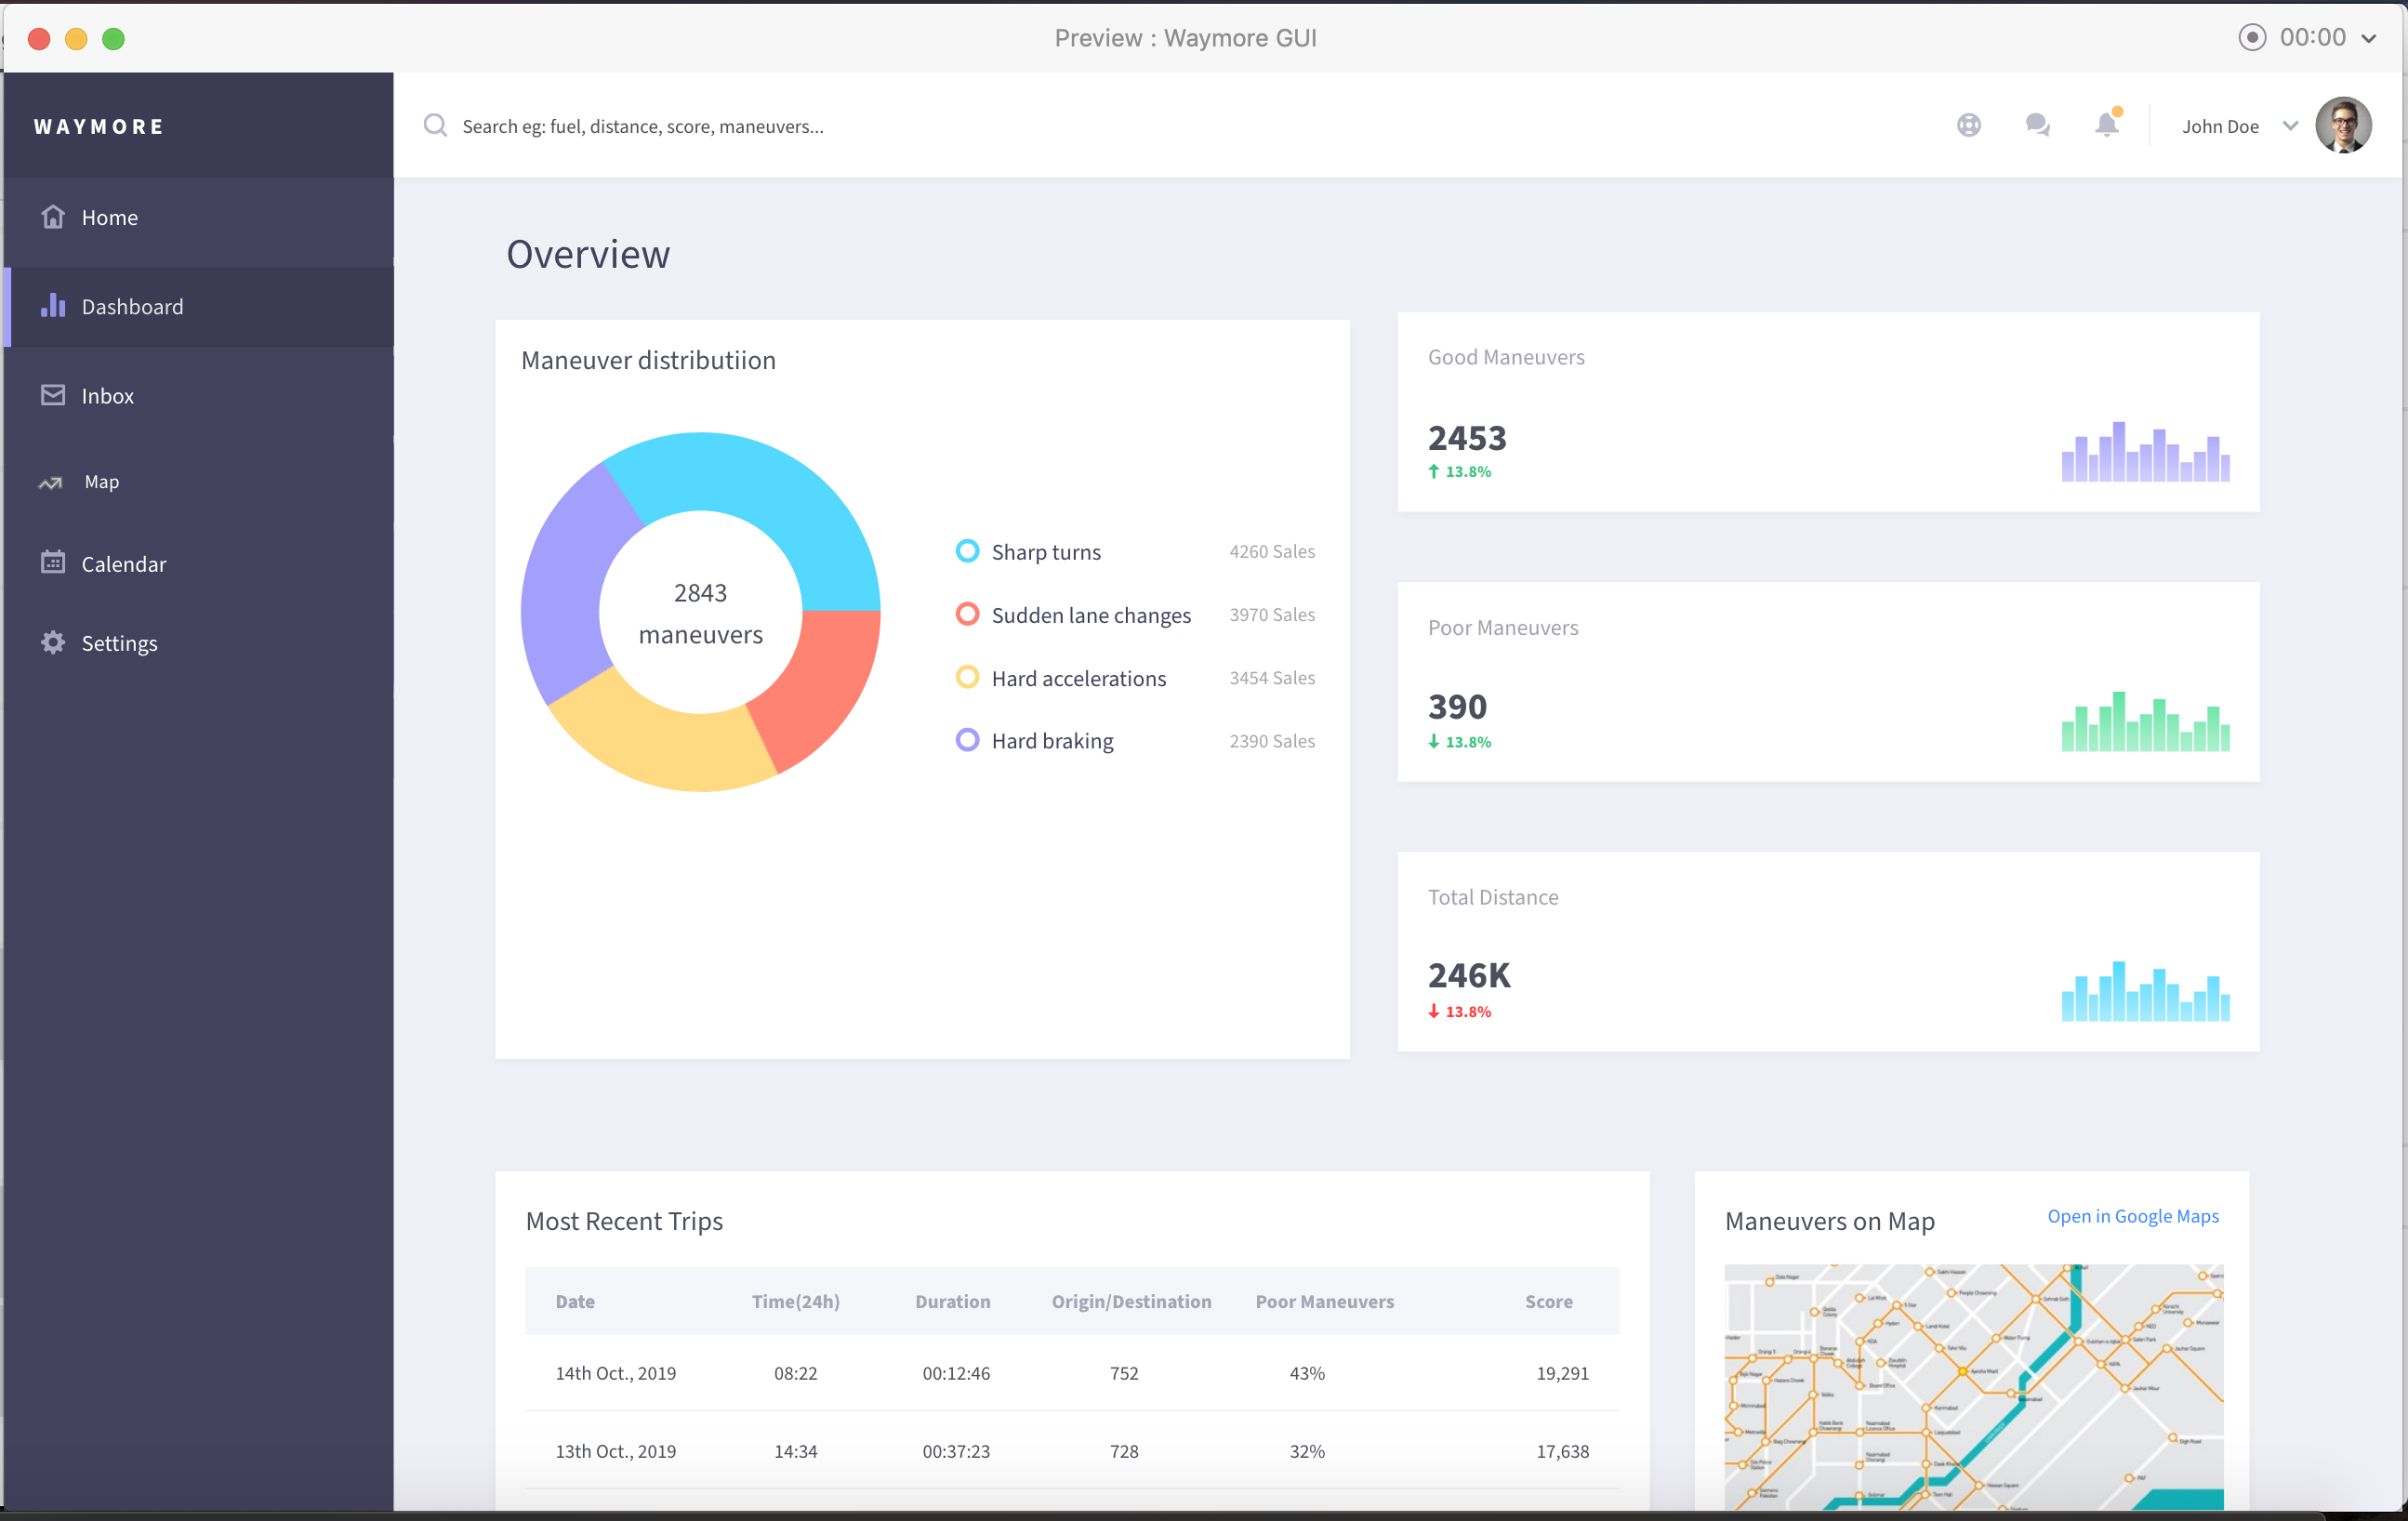
\includegraphics[width = 125mm, scale = 1]{images/2.png}

This screen is a dashboard that gives summary of the analysis to the users
\end{center}

\begin{center}

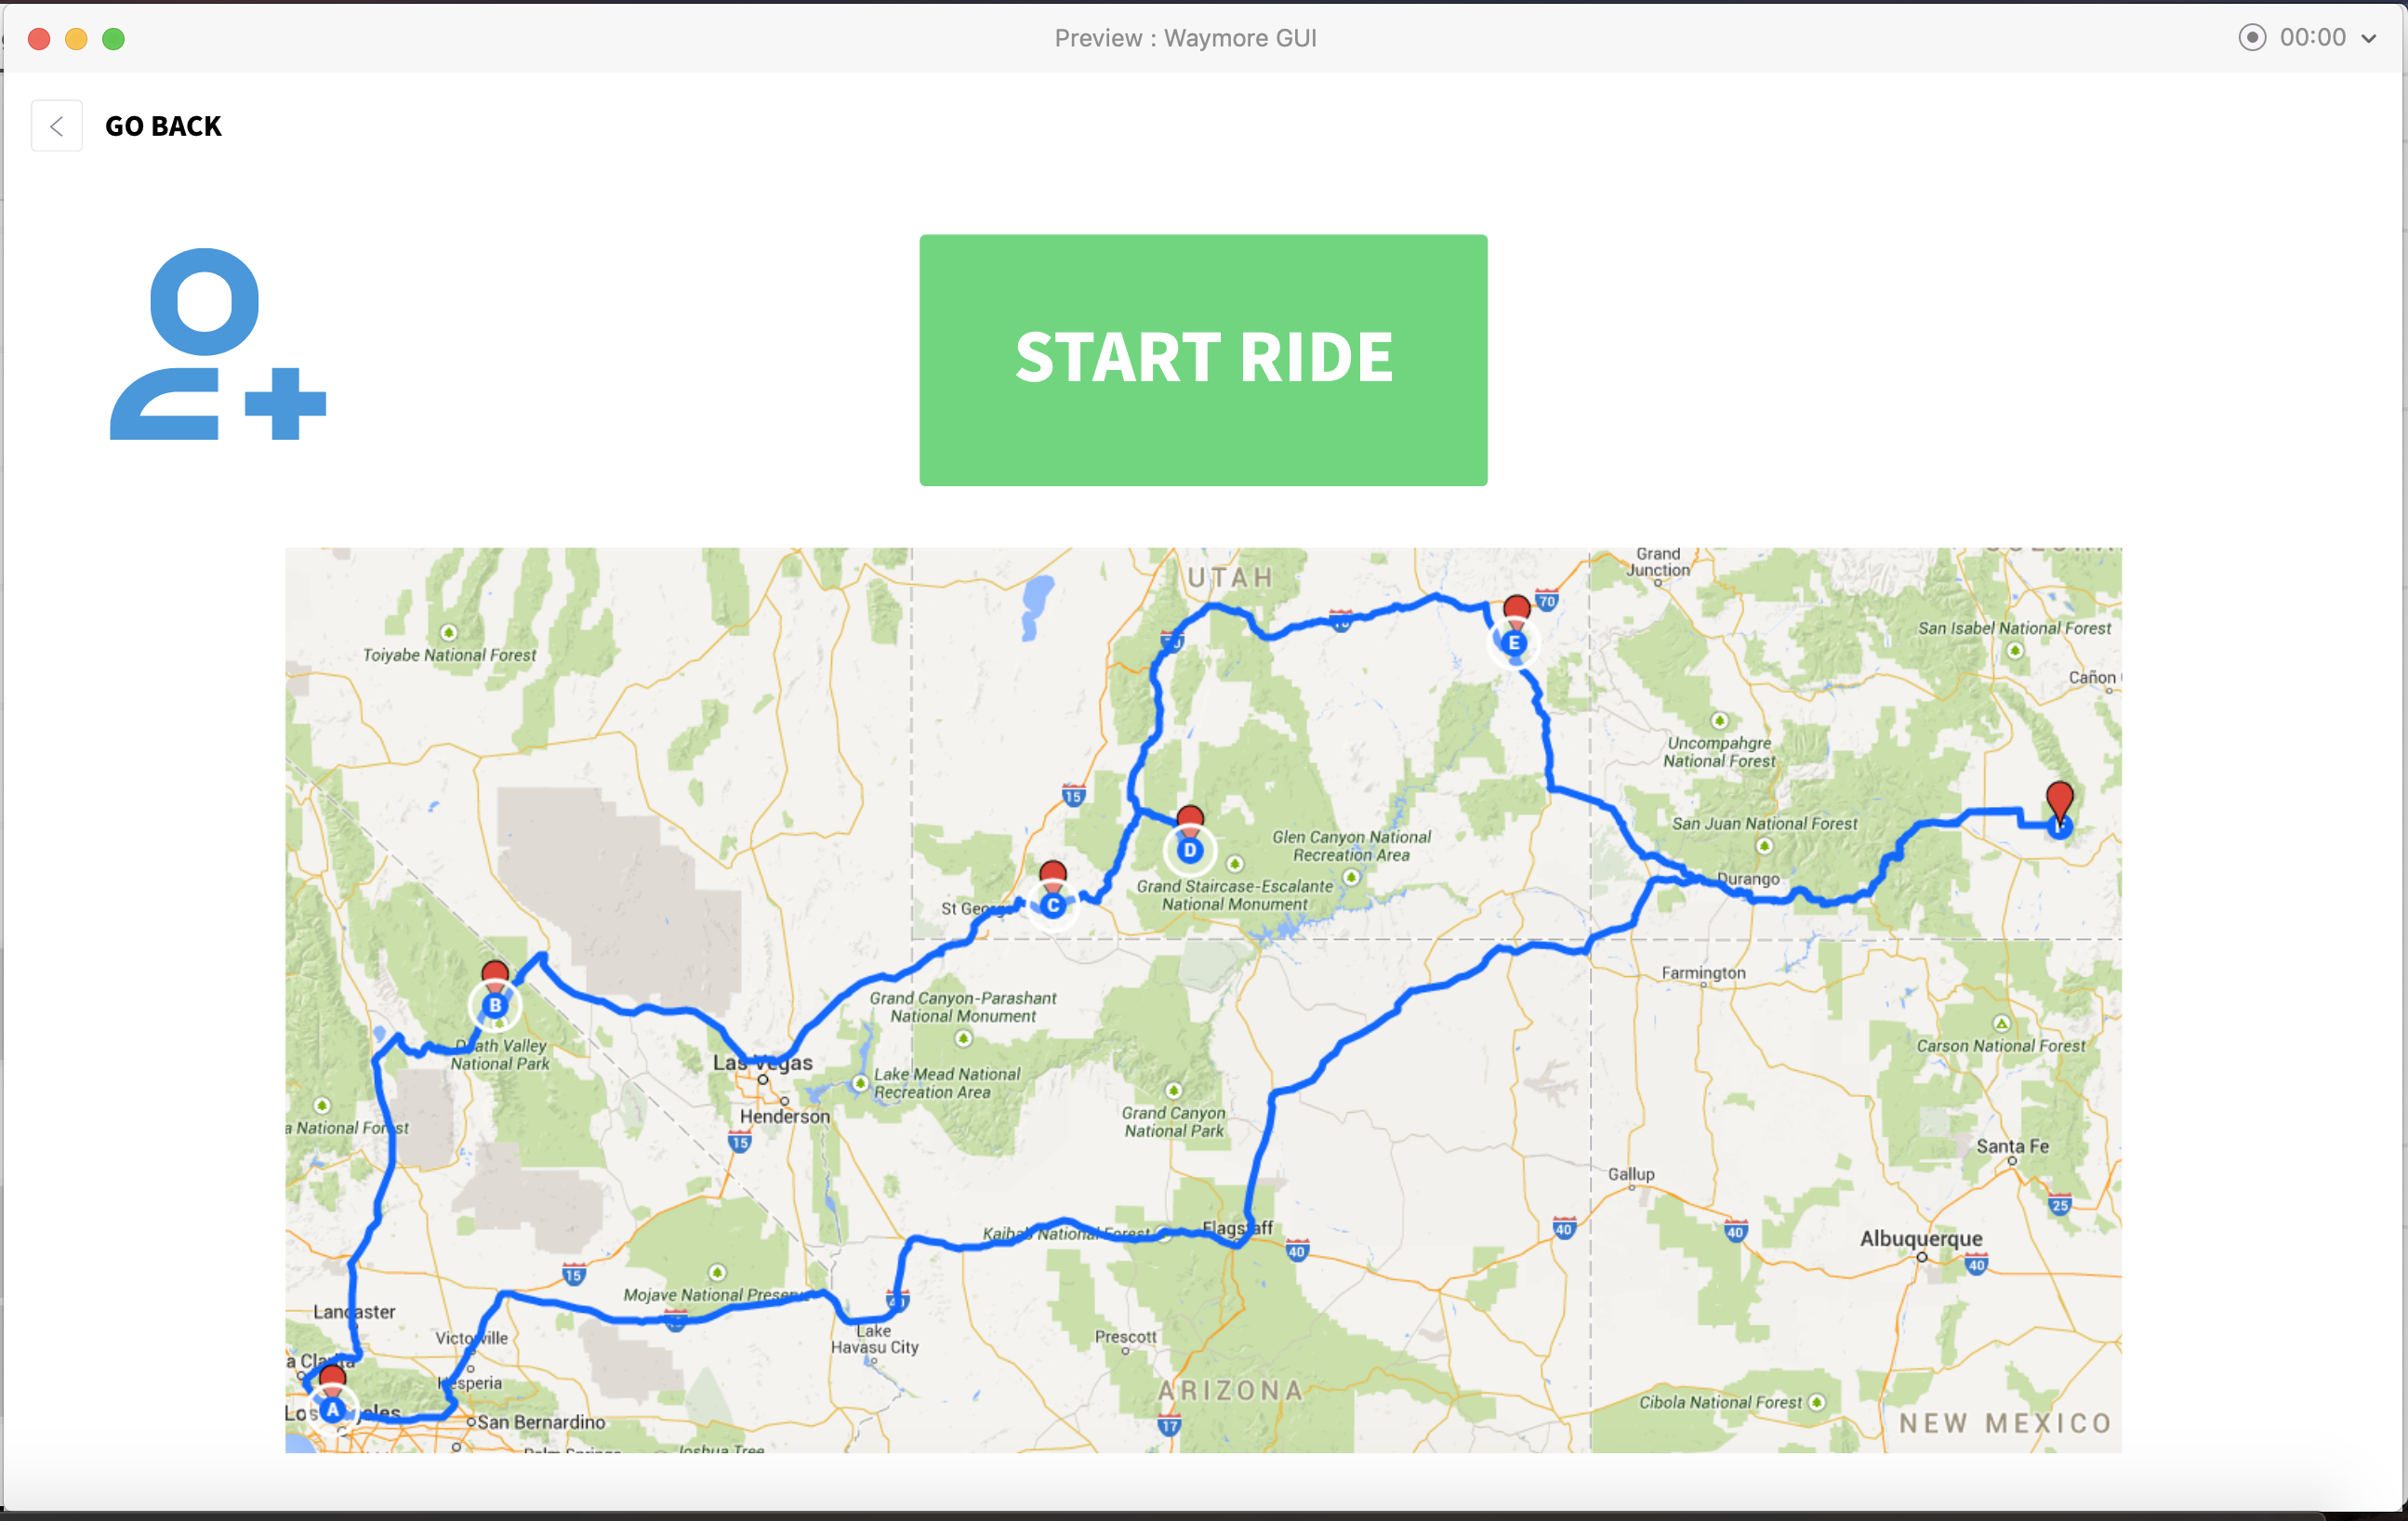
\includegraphics[width = 125mm, scale = 1]{images/3.png}

This screen shows the button for driver to start the ride\\

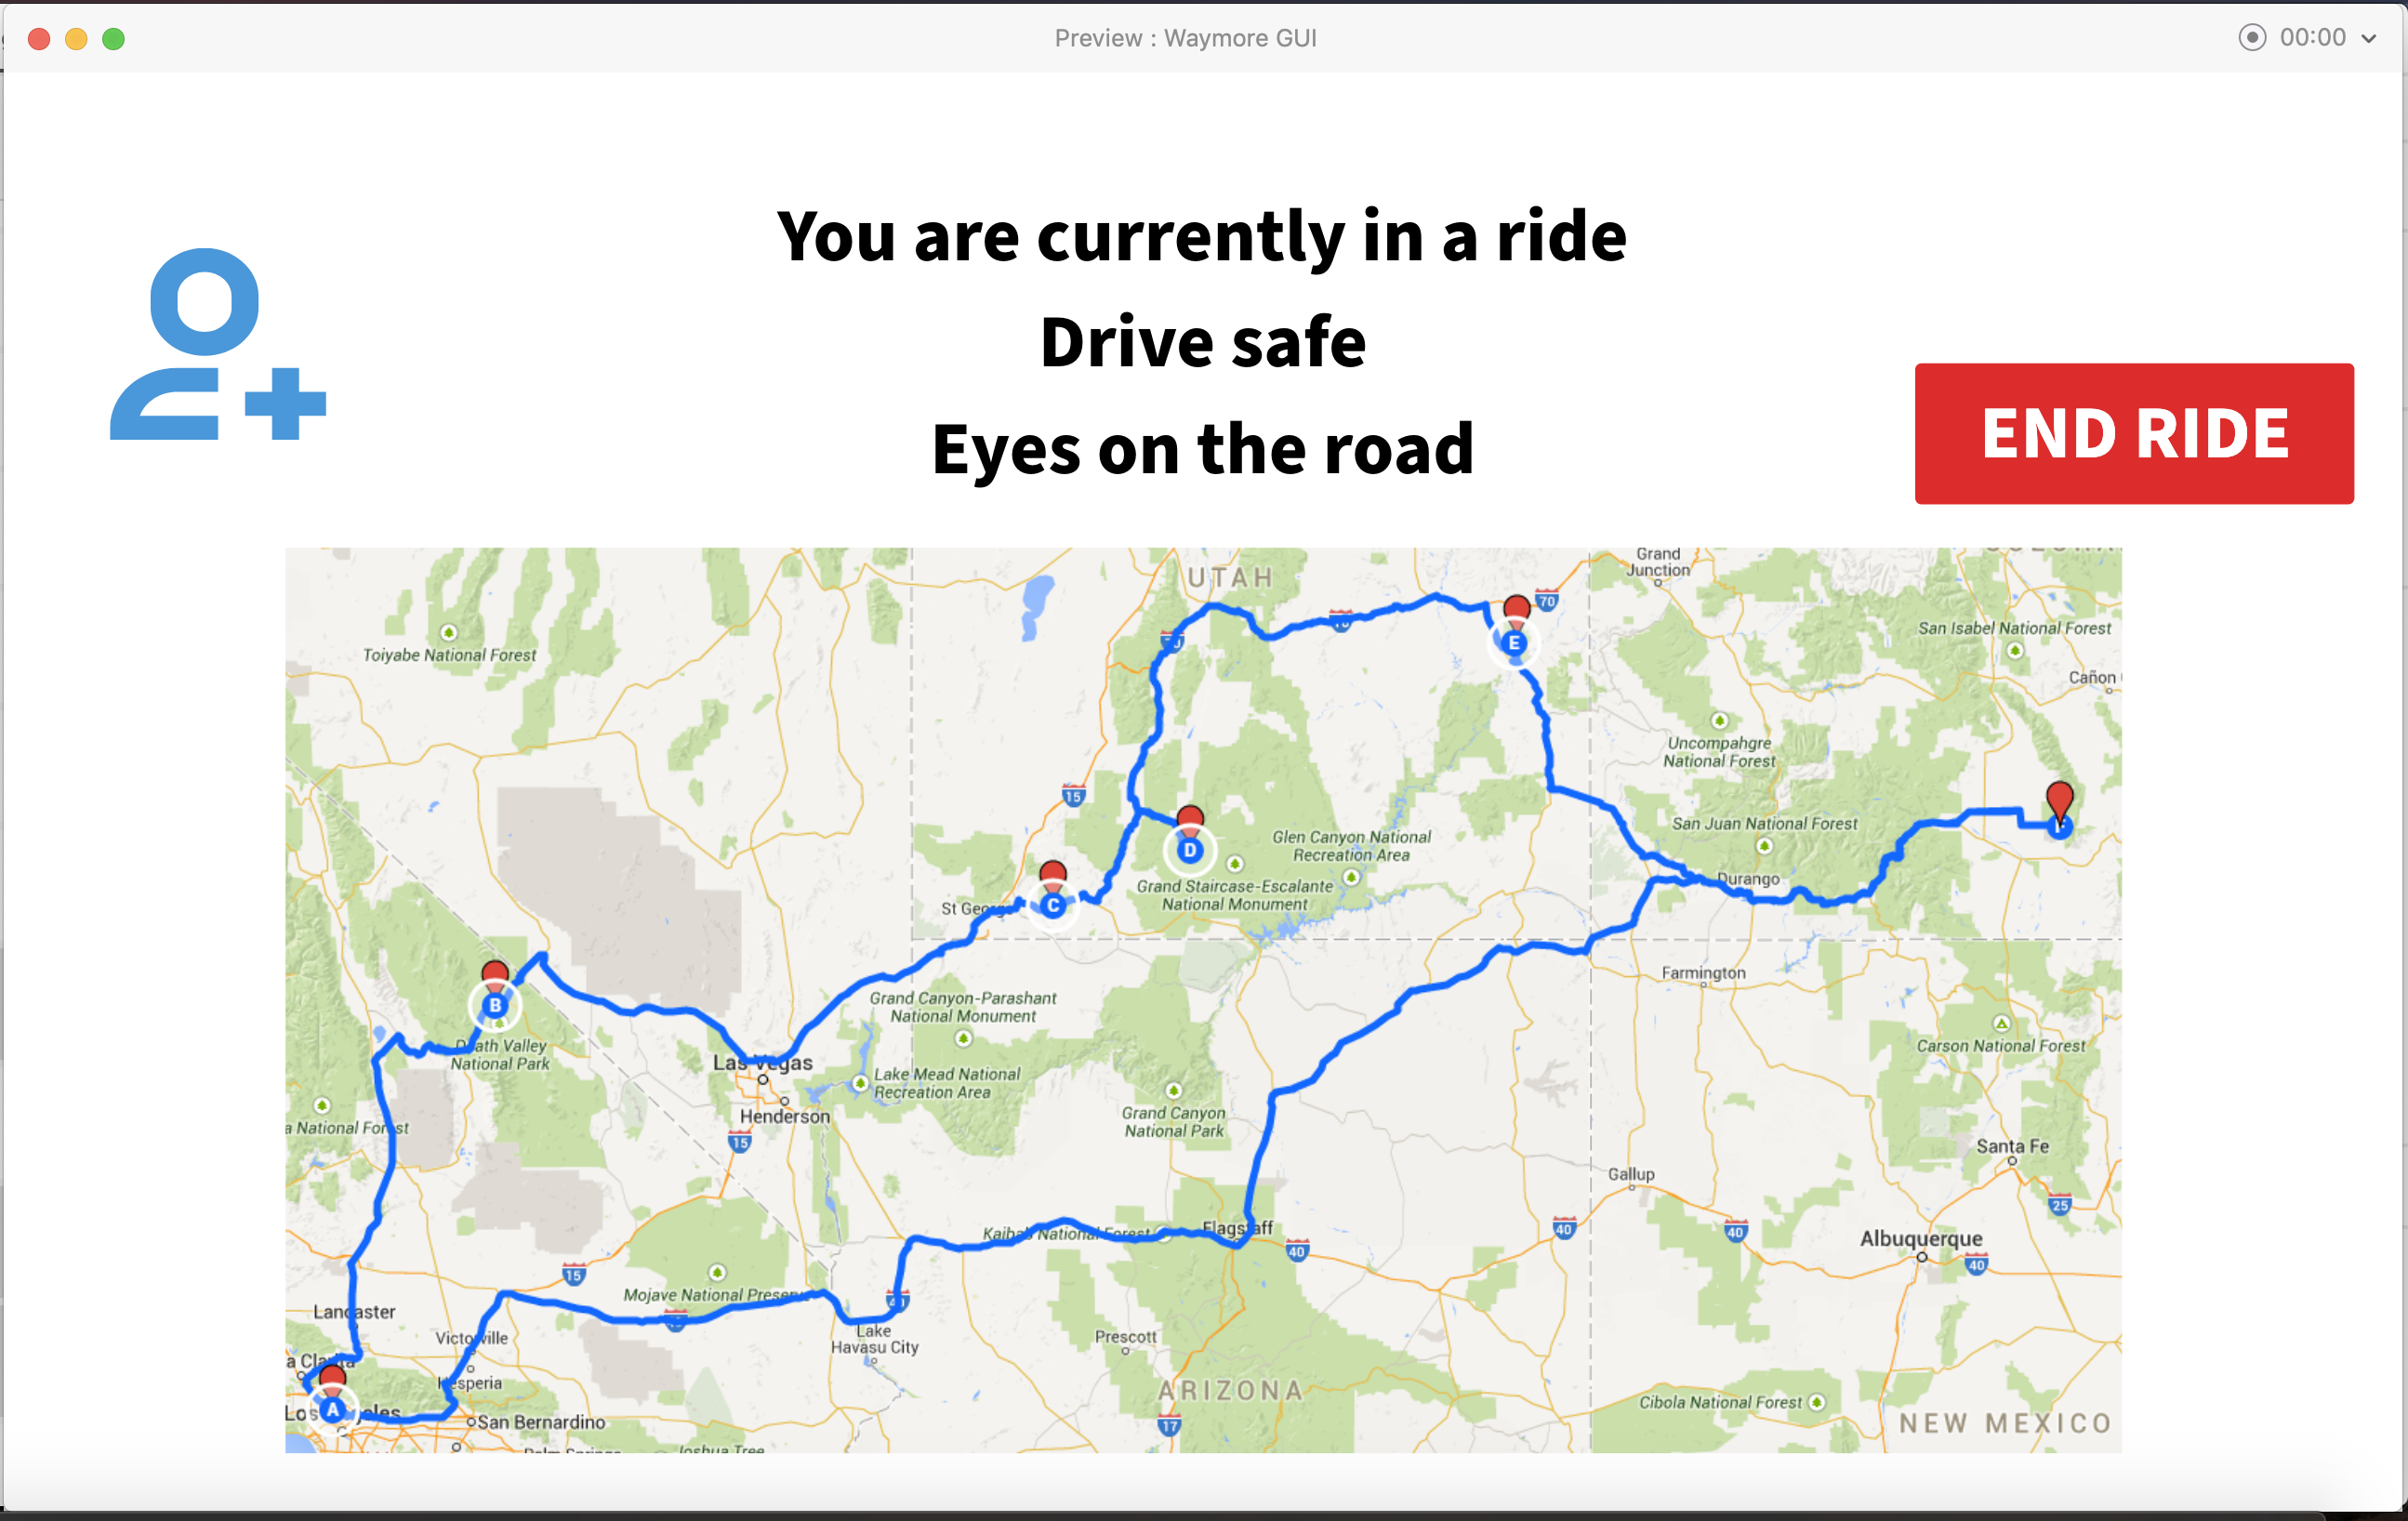
\includegraphics[width = 125mm, scale = 1]{images/4.png}

This screen shows the button for the driver to end the ride
\end{center}

\begin{center}
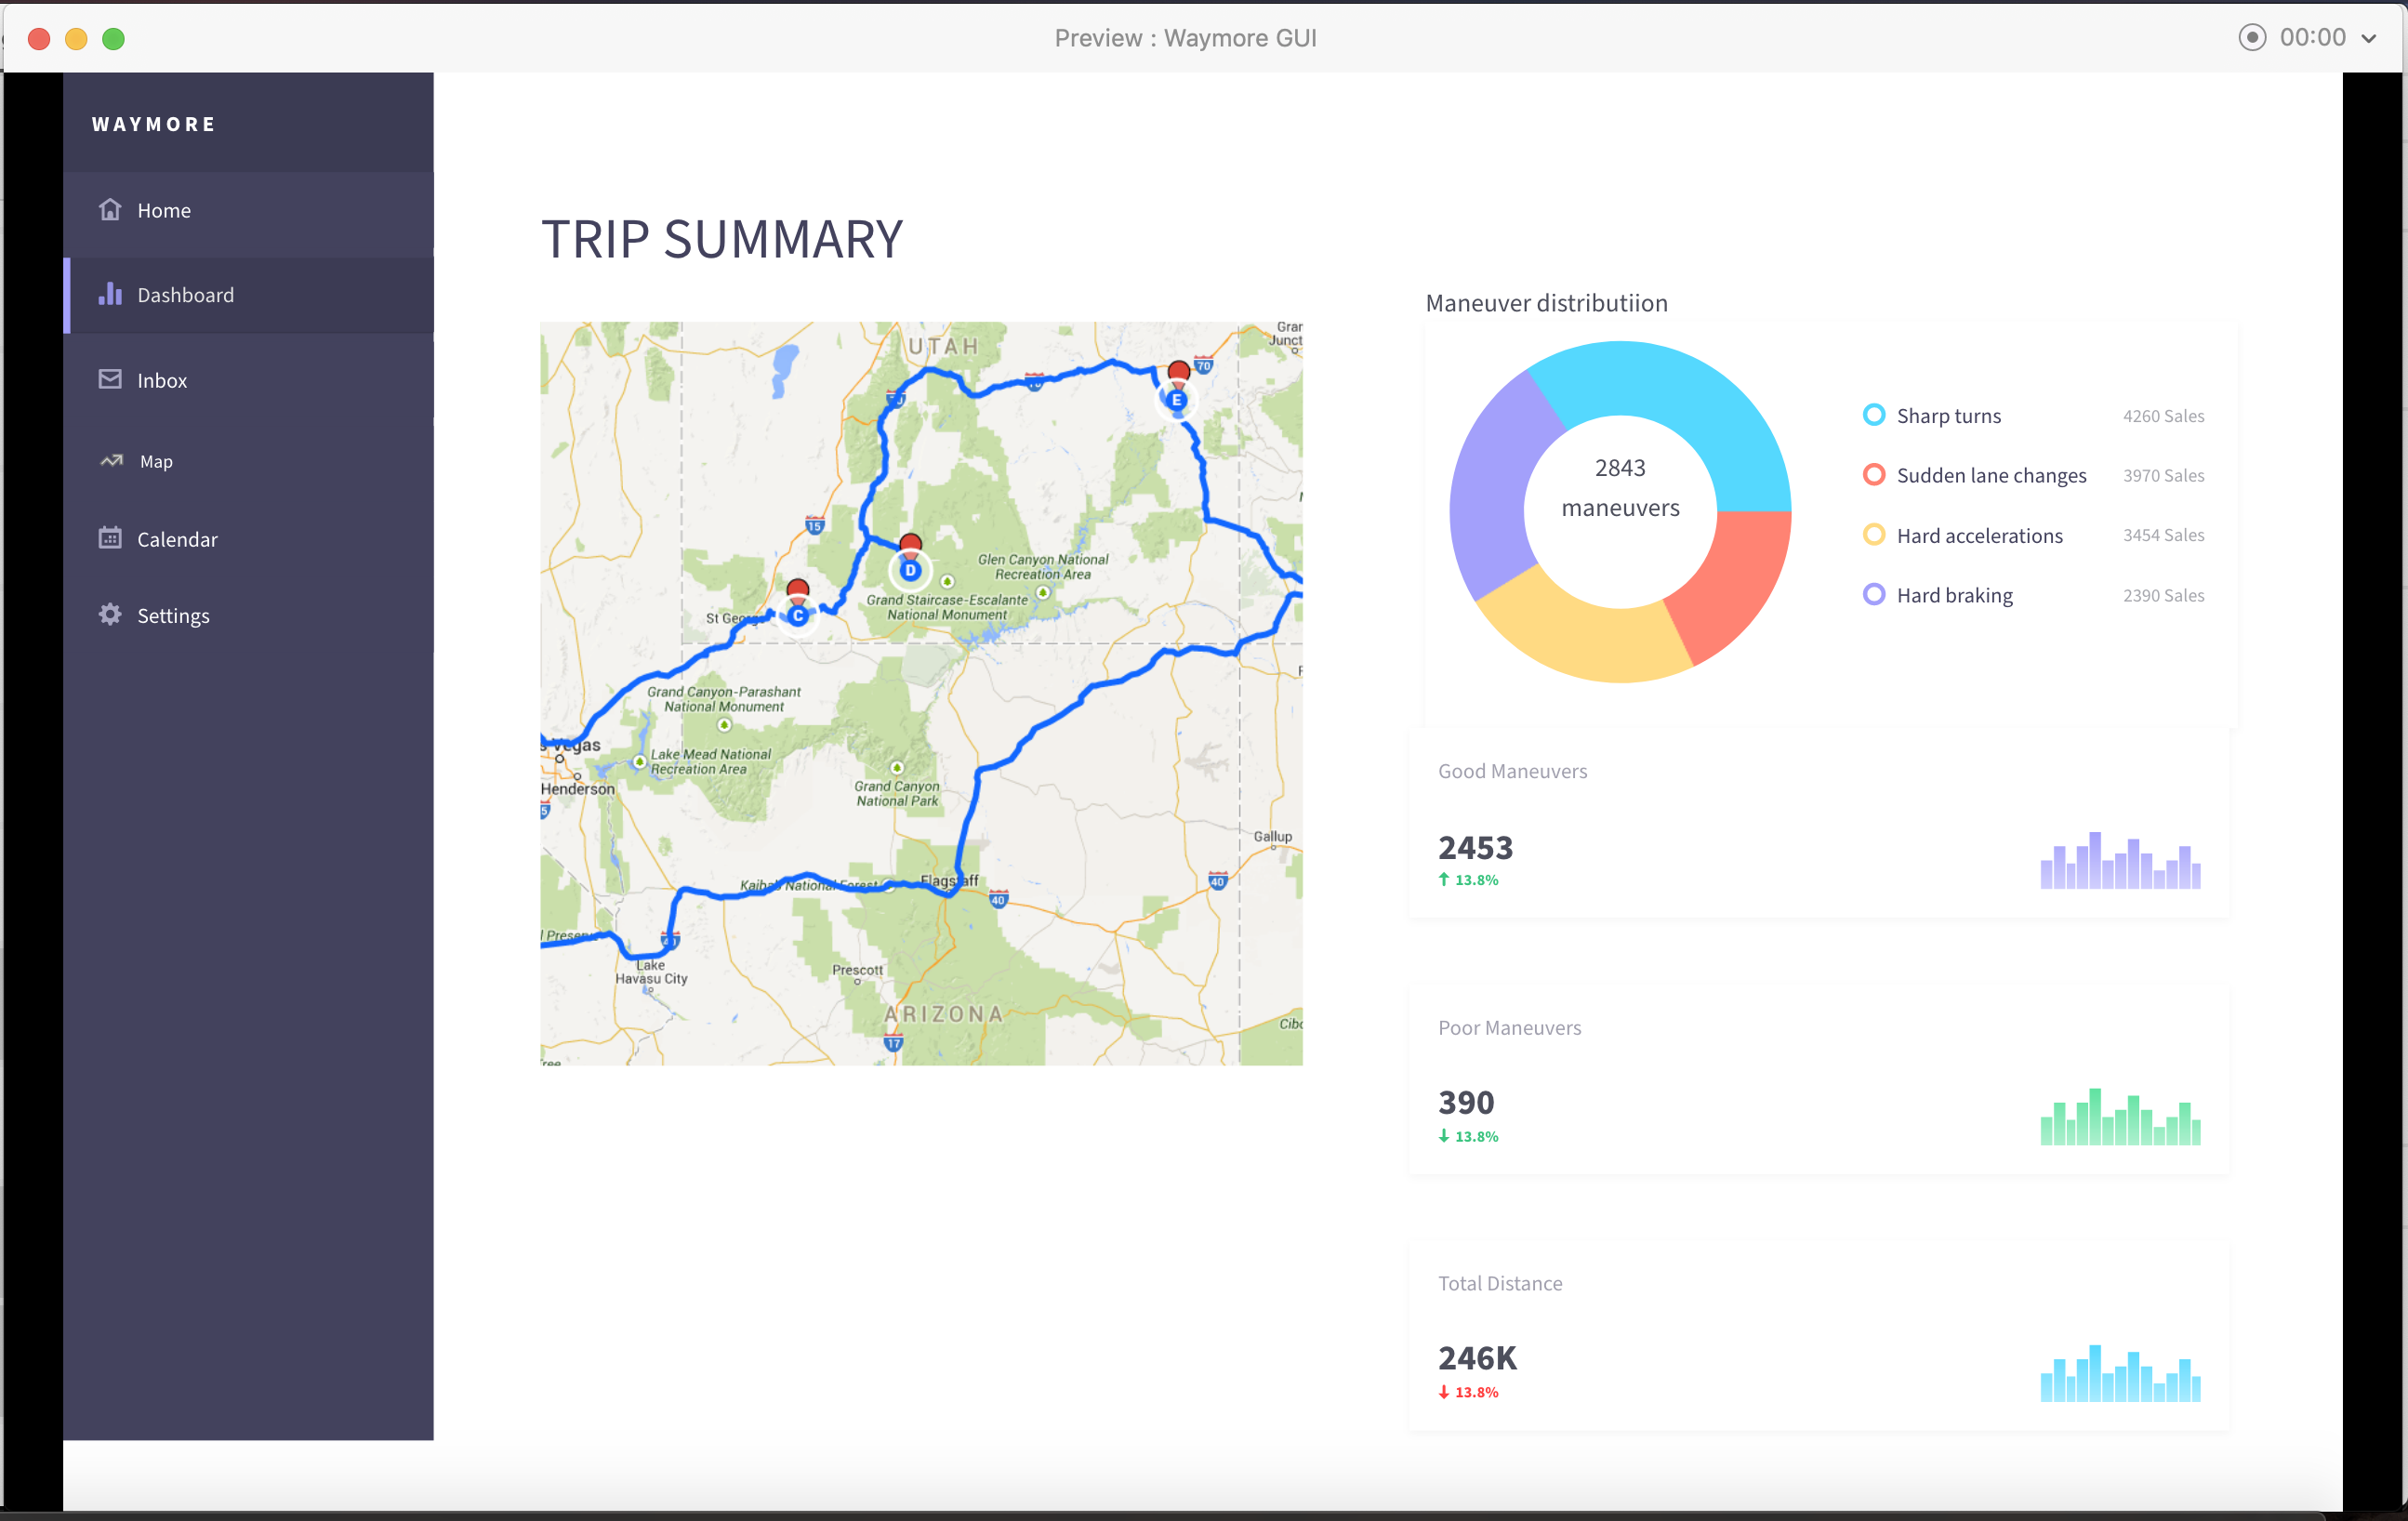
\includegraphics[width = 125mm, scale = 1]{images/5.png}

This screen shows the summary of the trip that is provided to the user at the end of each trip\\

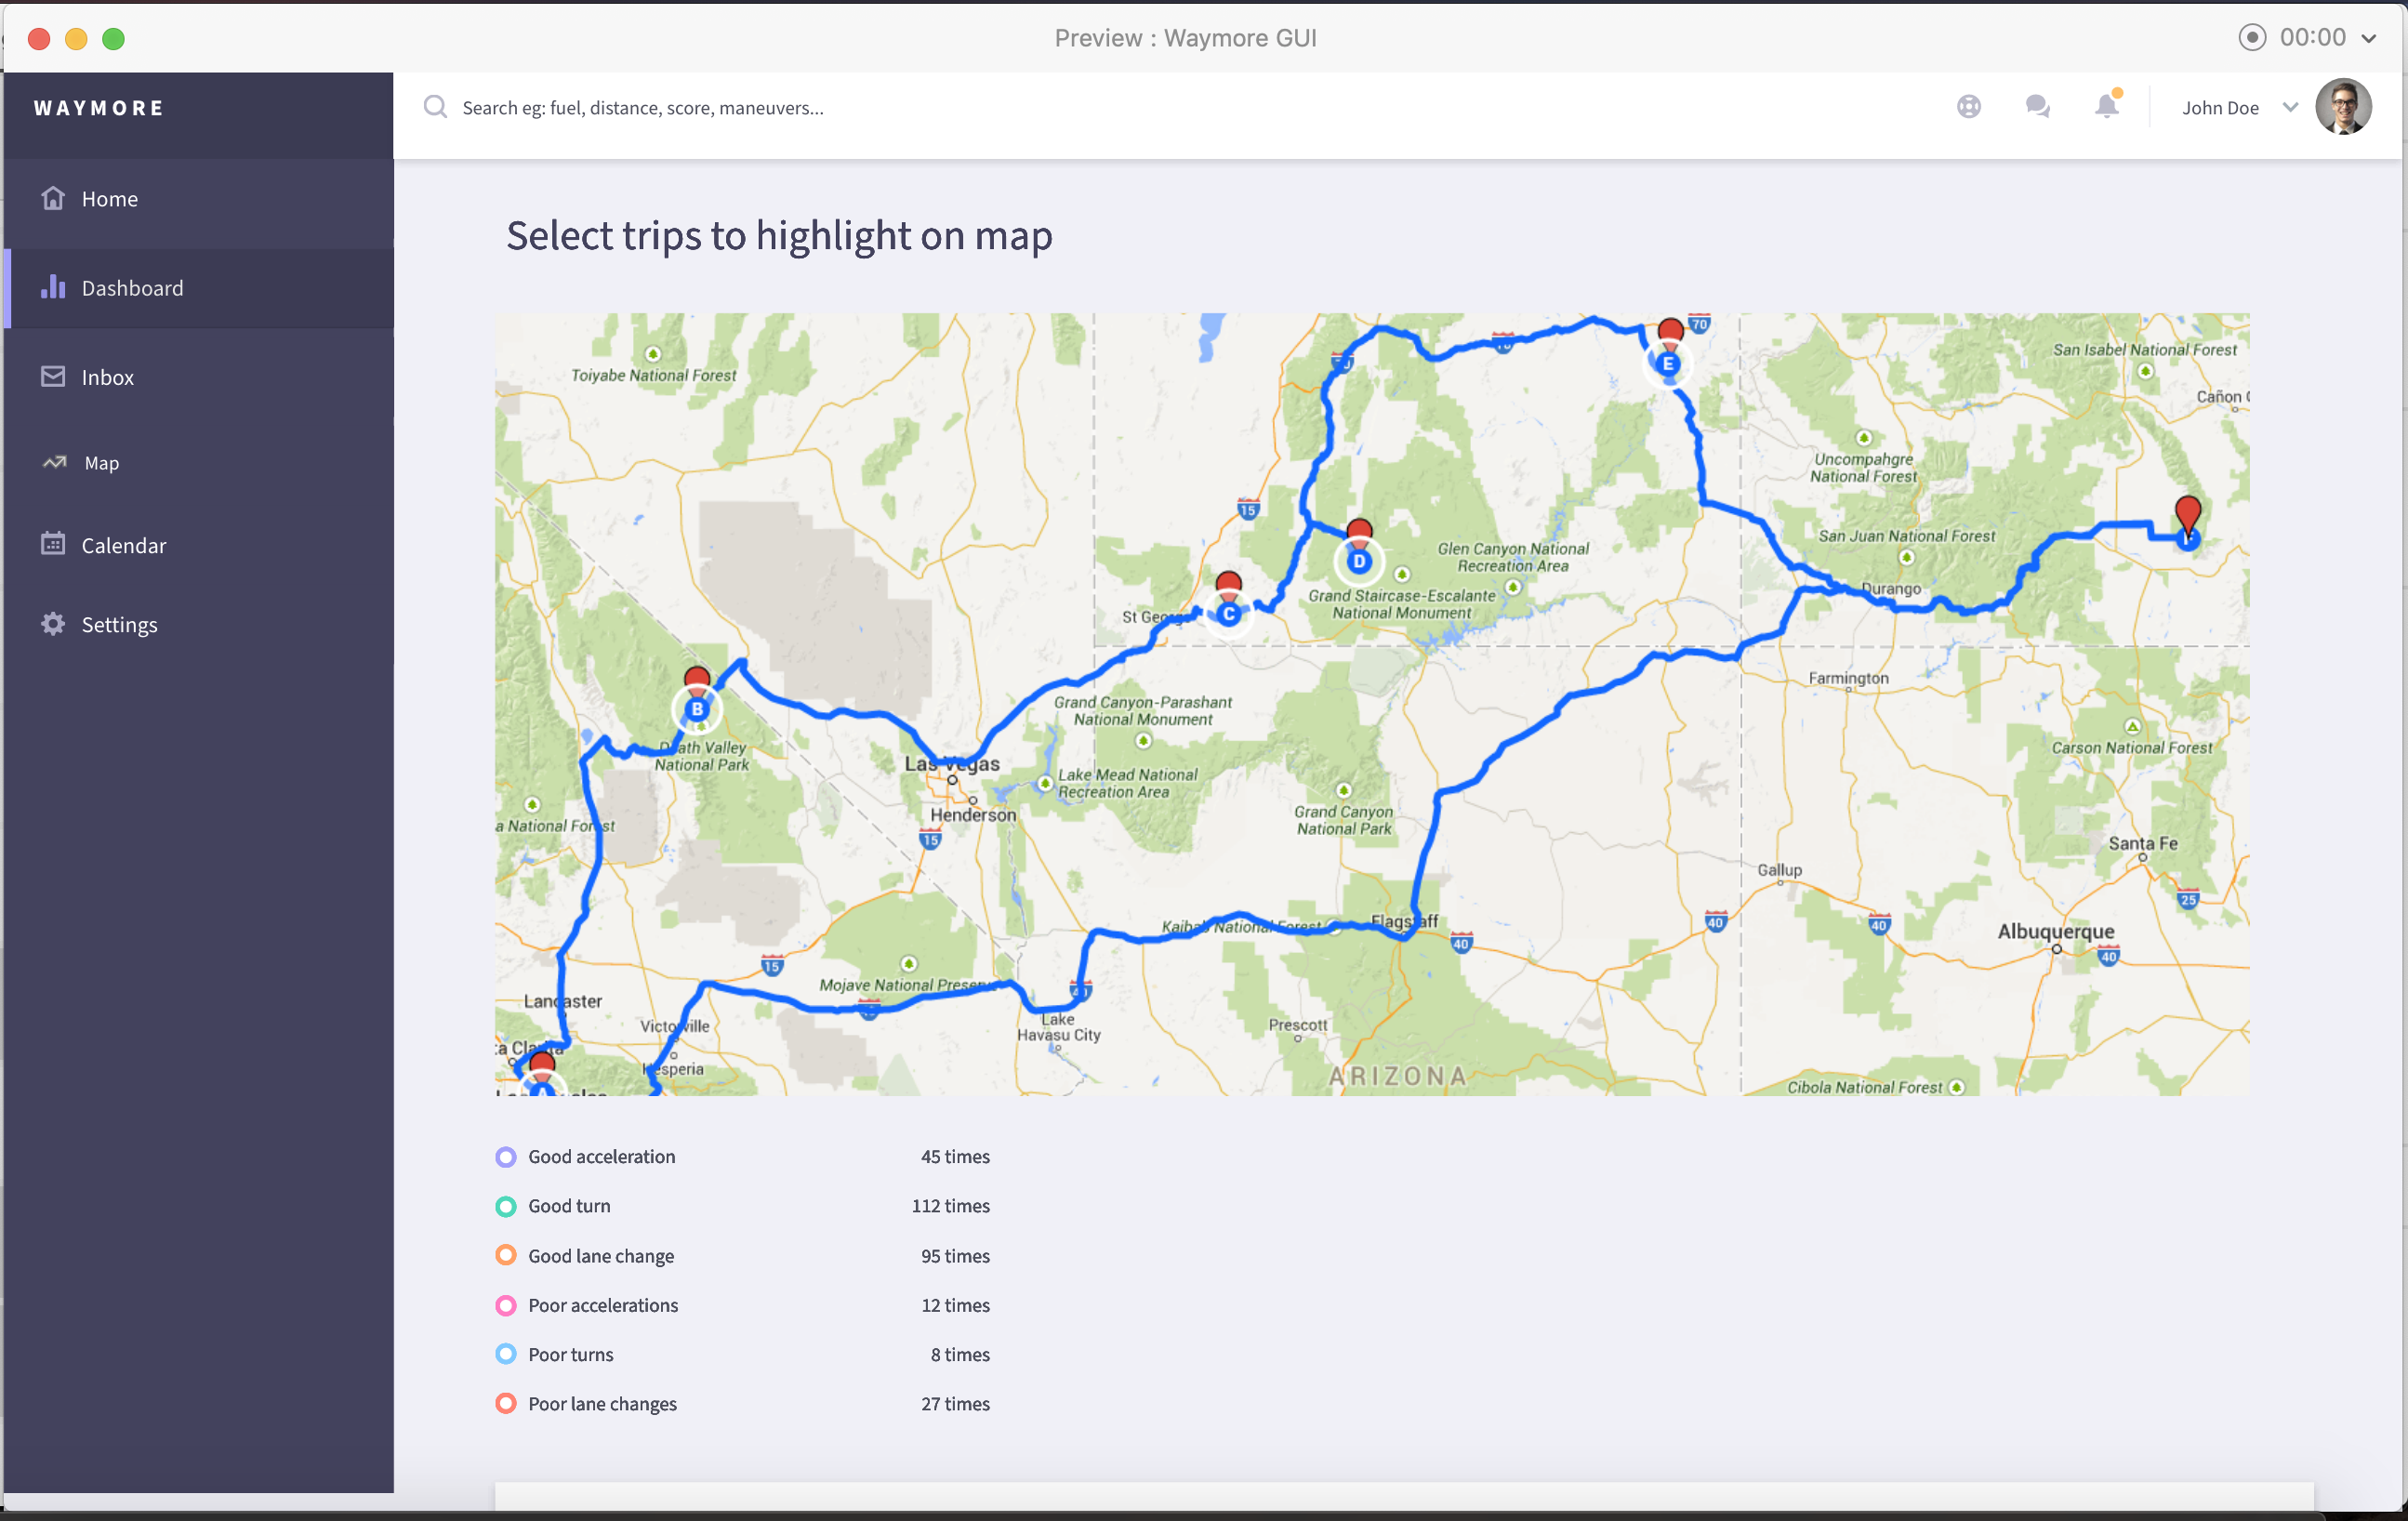
\includegraphics[width = 125mm, scale = 1]{images/7.png}

This screen shows the trips that have been carried out by the drivers allowing them to select and view details about a single trip\\
\end{center}

\subsection{Hardware Interface}
This section describes our project's specific hardware/network interfaces.

\begin{outline}

\1 Arduino UNO
\1 MPU6050 (IMU Unit)
\1 Adafruit ultimate GPS breakout

\end{outline}

\section{Use Cases}
This section presents detailed use cases of our system.

Use cases
\begin{outline}
\1 A Personal User:
\2 Sign up/Sign in
\2 Access dashboard $\rightarrow$ Total distance driven, average frequency of poor maneuvers, average frequency of good maneuvers
\2 View average score of day, week, month, year, custom range
\2 View all trips $\rightarrow$ trip profile
\2 Access trip profile for route (must), maneuver breakdown $\rightarrow$ each maneuver has time, location, logged against a graph, scoring process i.e. intensity and duration (information already displayed on graph) (nice)
\2 Badges? (nice?)

\1 A Fleet Employee:
\2 All the above (must)
\2 Segment trips via destinations, miles covered in specific states/cities/counties, positive reinforcement of all good maneuvers. (nice)

\1 Fleet Manager:
\2 All of the above (must)
\2 Access central dashboard where they can view 
\3 Each driver's profile (must)
\3 Each driver's trips' profiles (must)
\3 Cumulative fleet performance (must)
\3 Cumulative destinations visited/miles logged in area (nice)
\3 each maneuver breakdown (for focused efforts) for entire fleet (nice)
\2 Asset tracking (segment routes/active trips of a particular shipment (for eg: Twinkies en route to xyz location)), and how many trucks are active, which ones are in the depot, which ones are inactive for maintenance, which ones have been serviced between trips etc., mileage per vehicle (nice in entirety)
\end{outline}

\section{Datasets}
This section describes the specific dataset(s) used to build our system. An appropriate snapshot of the dataset(s) is also included. Futher details, when needed, are presented in the appendix\\

The Dataset that we are working with is called "Driver Behaviour Dataset" that is publicly available at this \textcolor{blue}{\href{https://github.com/jair-jr/driverBehaviorDataset}{link}}.This Dataset is optimal for our use case as it contains sensor readings for accelerometer, magnetometer and gyroscope; which are the sensors that we are primarily working with to classify different maneuvers.This dataset also comes with a paper that describes how the owners applied different Machine learning techniques (Support Vector Machine, Random Forest, Neural Nets) to this dataset to classify manuevers such as harsh acceleration, harsh braking etc. which can serve as a good guideline for us.

\begin{center}
\includegraphics[width = 150mm, scale = 1.5]{images/{sensordata.png}}
Snapshot of accelerometer data for one trip

\includegraphics[width = 75mm, scale = 1]{images/{truth.png}}\\
Snapshot of Event data for a single trip. Start time and End time are defined w.r.t trip start time.
\end{center}

\begin{center}
\includegraphics[width = 150mm, scale = 1.5]{images/{22.png}}
Visualization of Accelerometer x data for one trip

\includegraphics[width = 150mm, scale = 1.5]{images/{11.png}}
Visualization of time window on accelerometer x plot. (Time window represents a sharp right turn)
\end{center}


\section{System Diagram}
This diagram gives a high-level view of the different components of our system and the interactions between them. Each component and the particular tools/technologies/libraries used to build it are described.
\\

\begin{outline}


\end{outline}
\begin{center}
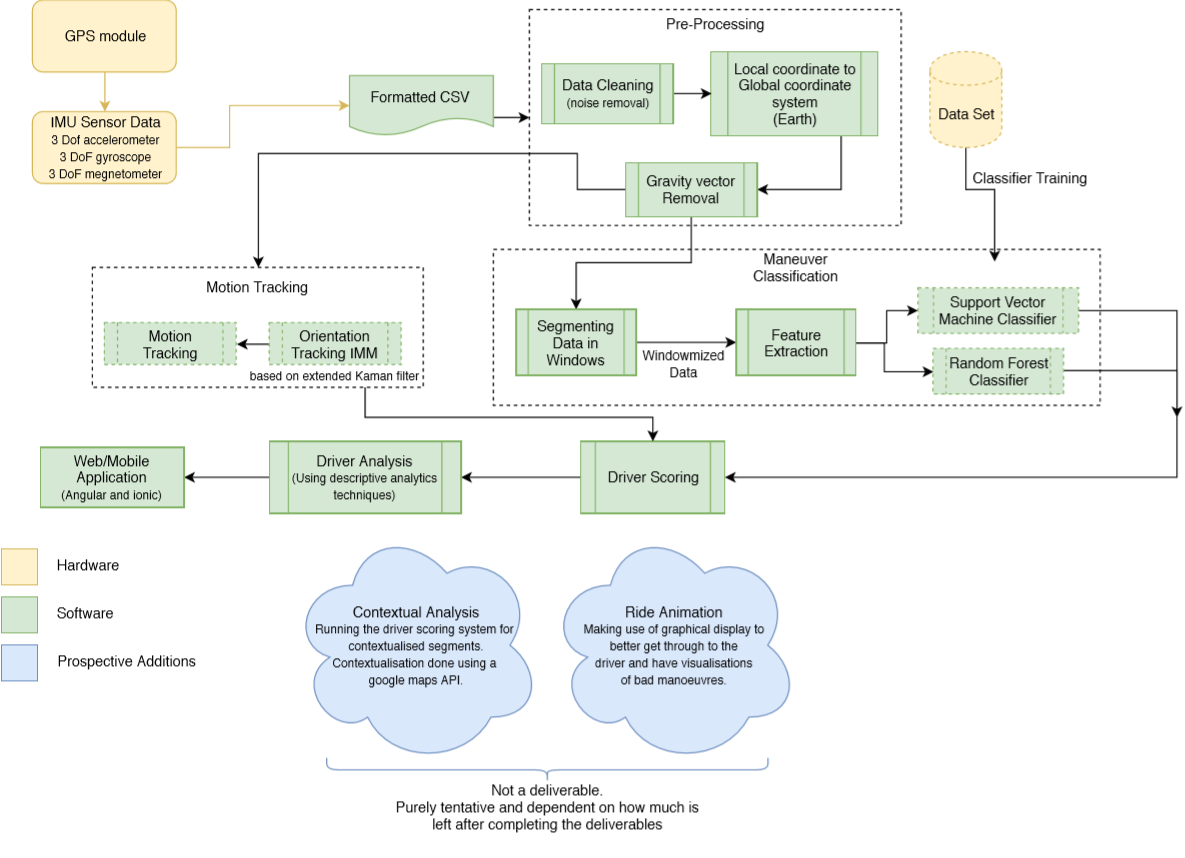
\includegraphics[width = 150mm, scale = 1.5]{images/system.png}
\end{center}

\begin{outline}
\1 The System Data Diagram is divided into 3 main heavy components. Pre-processing, Motion Tracking and Maneuver Classification. Pre-processing has to do with processing of the data our system acquires from our hardware modules and applying specific transformations; in order to convert the data in required csv format, filters; in order to clean the raw data of noise and other factors that are not relevant to our purpose, removal of the gravity factor from our 3DoF accelerometer for example. \\ 

\1 This processed data is fed separately feeded in both our modules, Motion Tracking and Maneuver classification. The Maneuver Classification module first segments our time-series data in windows of varying size, this windowmized data is then fed in for feature extraction. The windowmized data is run through several algorithms to fetch all relevant features like mean, max, and other relevant features. This featured and classified data is then used to feed in and train our classifiers, Support Vector Machine and Random Forrest, and then tested on the same. Motion Tracking module first achieves orientation tracking using an IMM, which runs based on extended Kalman filter. Having once achieved that, the same data is further fed into the Motion tracking module, which tracks the displacement with respect to the origin point, in a local coordinate system which can then be further used to transform to our desired coordinate frames.\\

\1 The results from both these modules, which are classified maneuvers with their sliding time windows, and a complete trajectory in 3 axis, are used based on already existing algorithms, to compute maneuvers and assign each one a score, which will in turn compute the score for the entire trip and over generations of a few trips, driver scoring will be achieved. This segmented, classified, and meaningful data about trips and the drivers will be further fed into the Driver Analytics module. And using this driver profile, the application will be developed.
\end{outline}